\documentclass[11pt,answers]{exam}

\usepackage{etex}
\usepackage{amssymb,amsmath,multicol} %<-- InWorksheetExam1 i also have fancyhdr,

\usepackage[metapost]{mfpic}
\usepackage[pdftex]{graphicx}

\usepackage{pst-plot}
\usepackage{pgfplots}
\pgfplotsset{compat=1.9}

\usepackage{tikz}
\usepackage{tkz-2d}
\usepackage{tkz-base}
\usetikzlibrary{calc}

\usepackage[inline]{enumitem}
\usepackage{refcount}%<-- non in WorksheetExam1

%\renewcommand{\headrulewidth}{0pt}

\newcommand{\vasymptote}[2][]{
    \draw [densely dashed,#1] ({rel axis cs:0,0} -| {axis cs:#2,0}) -- ({rel axis cs:0,1} -| {axis cs:#2,0});
}

\addpoints
%\printanswers
\noprintanswers

\opengraphsfile{TestOfParts}

\begin{document}
\extrawidth{-0.3in}
\pagestyle{headandfoot}

\setlength{\hoffset}{-.25in}

\extraheadheight{-.4in}
\runningheadrule
\firstpageheader{\bfseries {MATH1-UC 1171}}{ \bfseries {Exam 1 }}{\bfseries {3/10/2015}} 



\firstpagefooter{\bfseries{}}{}{} 


\runningheader{\bfseries {}}%
              {\bfseries {}}%
              {Page \thepage\ 
							of \numpages 
							}
\runningfooter{} %%&&CHANGED
                {}
                {Points earned: \hbox to 0.5in{\hrulefill}
                 out of  \pointsonpage{\thepage} points}
                 
						

\vspace*{0.7cm}
\hbox to \textwidth { \scshape {Name:} \enspace\hrulefill}
\vspace{0.2in}

\begin{itemize}
	\item This exam contains \numpages\ pages, including this cover page and the blank last page which you can tear out and use as scrap paper. Enter
your name on the top of this page, and put your initials
on the top of every page. Please note that I will not grade anything that you write on the last (blank) page.

%\item Please read the instructions for each individual problem carefully. Try not to overthink a problem and read between the lines! Take your time to solve each problem, and don't rush to finish!
%\item Write legibly and clearly label your answers. If I cannot read your solution to a problem, the problem will receive a score of zero.
\item Calculators may not be used in this exam. You may use your note-card with fomulas/examples. 

\item Please write your name on your note-card and include it in your exam. If you do not have a note-card, please write {\textit {no note-card}} on this page.
\item Turn off all phones and computers, and remove all headphones.

\end{itemize}

For the problems where you are required to show your work, the following rules apply:\\

\begin{minipage}[t]{3.7in}
\vspace{0pt}
\begin{itemize}

\item \textbf{Write in complete sentences}, explaining your calculations, graphs and tables. If you draw a graph, you must label the axes, include tick marks and include units both on the horizontal and vertical axis. If you are asked to explain in practical terms, then your explanation cannot contain math symbols or formulas.
\item \textbf{Use the methods described in this course} as part of your explanations: for example, you cannot use derivatives to find the peaks and valley of a function.

\item \textbf{Organize your work}, neatly and legibly in
the space provided. Work that is disorganized and difficult to read will not receive full credit.  

\item \textbf{A correct answer, unsupported by calculations, explanation,
or algebraic work will receive no credit}; an incorrect answer supported
by  calculations and explanations may receive
partial credit.


\item \textbf{If you need more space}, use the back of the pages; clearly indicate when you have done this.
\end{itemize}

Do not write in the table to the right.
\end{minipage}
\hfill
\begin{minipage}[t]{2.3in}
\vspace{0pt}
%\cellwidth{3em}
\gradetablestretch{2}
\vqword{Pages}
\addpoints % required here by exam.cls, even though questions haven't started yet.	
\combinedgradetable[v][pages]  % Use [pages] to have grading table by page instead of question

\end{minipage}
\newpage

%\bigskip

%\begin{center}
%\gradetable[v][pages]
%\end{center}

%\newpage

\pointpoints{Point}{Points}

\begin{questions}


\addpoints
\qformat{Question \thequestion\dotfill
         {(\pointsofquestion{\arabic{question}} \points)}}

\bonusqformat{Bonus Question \thequestion\dotfill
         {(\bonuspointsofquestion{\arabic{question}} \points)}}        
        
%%%%%%%%%%%%%%%%

\question 

Consider the polynomial: $\displaystyle y=1-9x^8$. Are the following statements true or false?

\begin{parts}
\part[1] If $x\to -\infty$, then $y\to -\infty$
\begin {oneparchoices}
\choice True \choice False
\end{oneparchoices}
\part[1] If $x\to \infty$, then $y\to -\infty$
\begin {oneparchoices}
\choice True \choice False
\end{oneparchoices}
\end{parts}


\question The shaded region in the graph shown below represents a feasible region.

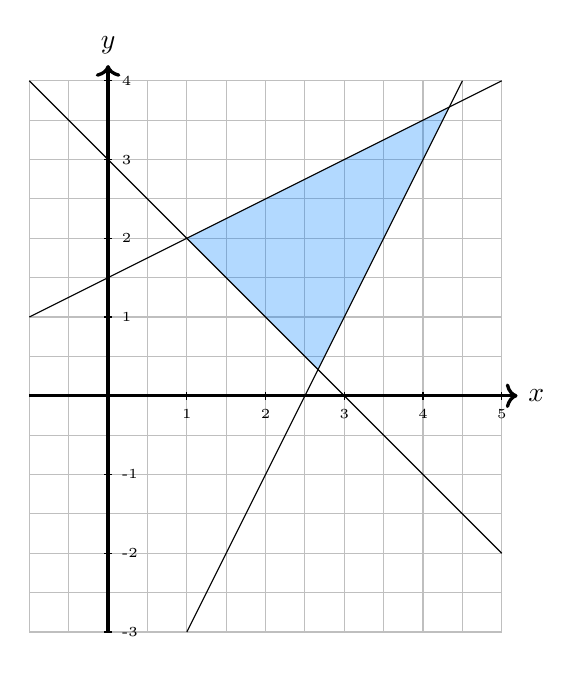
\begin{tikzpicture}

    \draw[gray!50, thin, step=0.5] (-1,-3) grid (5,4);
    \draw[very thick,->] (-1,0) -- (5.2,0) node[right] {$x$};
    \draw[very thick,->] (0,-3) -- (0,4.2) node[above] {$y$};

    \foreach \x in {1,...,5} \draw (\x,0.05) -- (\x,-0.05) node[below] {\tiny\x};
    \foreach \y in {1,...,4} \draw (-0.05,\y) -- (0.05,\y) node[right] {\tiny\y};
    \foreach \y in {-3,...,-1} \draw (-0.05,\y) -- (0.05,\y) node[right] {\tiny\y};

    \fill[blue!50!cyan,opacity=0.3] (8/3,1/3) -- (1,2) -- (13/3,11/3) -- cycle;

    \draw (-1,4) -- node[below,sloped] {} (5,-2);
    \draw (1,-3) -- (3,1) -- node[below left,sloped] {} (4.5,4);
    \draw (-1,1) -- node[above,sloped] {} (5,4);

\end{tikzpicture}

\begin{parts}
\part[1] Is this statement true or false?  One of the inequalities which define the feasible region is $\displaystyle y\leq -x+3$. 
\begin{oneparchoices}
\choice True \choice False
\end{oneparchoices}
\part[1] Is this statement true or false?  One of the inequalities which define the feasible region is $\displaystyle y\geq 0.5x+3$. 
\begin{oneparchoices}
\choice True \choice False
\end{oneparchoices}
\part[1] Is this statement true or false? If the objective function is $\displaystyle M=200-x-y$, then  the maximum of $M$ in the feasible region cannot be at $(3,2)$.
\begin{oneparchoices}
\choice True \choice False
\end{oneparchoices}
\end{parts}



\question

Which of these functions are polynomial functions?

\begin{parts}
\part[1] $\displaystyle y=\frac{4+x^3}{x}$
\begin{oneparchoices}
\choice Polynomial \choice Not polynomial
\end{oneparchoices}
\part[1] $\displaystyle y=\sqrt{x^2+2x+3}$
\begin{oneparchoices}
\choice Polynomial \choice Not polynomial
\end{oneparchoices}
\part[1] $\displaystyle y=|x|$
\begin{oneparchoices}
\choice Polynomial \choice Not polynomial
\end{oneparchoices}
\part[1] $\displaystyle y=x^2+\frac{2}{3}x+\sqrt{3}$
\begin{oneparchoices}
\choice Polynomial \choice Not polynomial
\end{oneparchoices}
\end{parts}

\end{questions}

\end{document}                 